\documentclass[a4paper]{exam}
\usepackage{graphicx}
\usepackage{cmbright}
\usepackage{caption}
\usepackage{subcaption}
\usepackage{multirow}
\usepackage{siunitx}
\usepackage{svg}

\firstpageheader{EE5907}{CA2}{\today}
\runningheader{EE5907}{CA2 (Continued)}{\today}
\footer{}{\thepage}{}

\graphicspath{ {figures/} }

\newcommand\percentage[2][round-precision = 2]{% default precision: 2
    \qty[round-mode = places,
        scientific-notation = fixed, fixed-exponent = 0,
        output-decimal-marker={.}, #1]{#2e2}{\percent}%
}


\begin{document}
\begin{questions}
    \question PCA based data distribution visualizations

    Let the data matrix $\mathbf{X}$ be of $n \times p$ size.\\
    First, perform SVD:
    \begin{equation}
        \mathbf{X}=\mathbf{USV^T}
    \end{equation}
    The columns of $\mathbf{US}$ are the principal components and the columns of $\mathbf{V}$ are the eigenfaces.\\
    For the principal components, only calculation for the highest dimension is necessary. For reduction to
    dimension $k$, the first $k$ principal components can be obtained from the first $k$ columns of
    $\mathbf{U}$ and the diagonal matrix formed by the first $k$ values along the diagonal of $\mathbf{S}$.

    \begin{figure}[h]
        \centering
        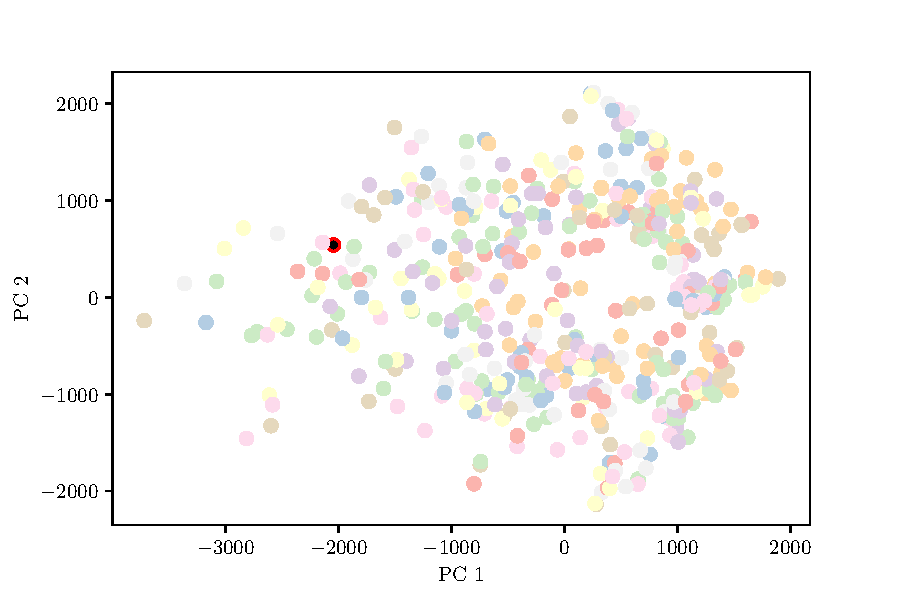
\includegraphics[width=0.75\textwidth]{pca_2d}
        \caption{PCA projected data vector in 2D.}
        \label{fig:pca_2d}
    \end{figure}

    \begin{figure}[ht]
        \centering
        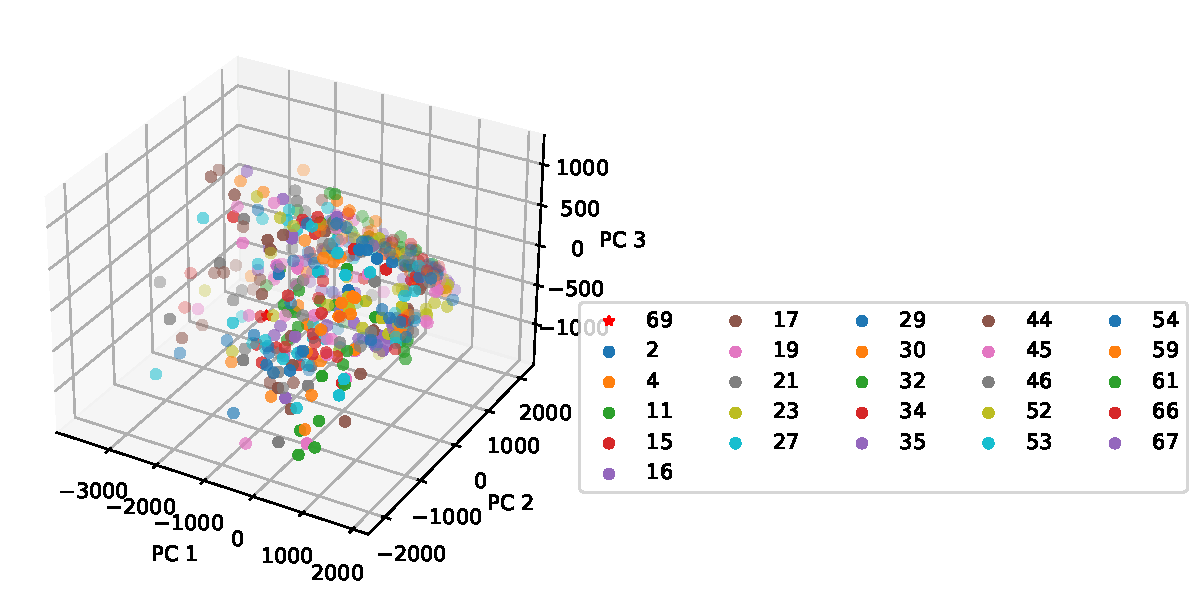
\includegraphics[width=0.75\textwidth]{pca_3d}
        \caption{PCA projected data vector in 3D.}
        \label{fig:pca_3d}
    \end{figure}

    \begin{figure}[ht]
        \centering
        \begin{subfigure}[b]{0.3\textwidth}
            \centering
            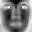
\includegraphics[width=\textwidth]{eigenface0}
            \caption{eigenface 0}
            \label{fig:eigenface0}
        \end{subfigure}
        \hfill
        \begin{subfigure}[b]{0.3\textwidth}
            \centering
            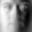
\includegraphics[width=\textwidth]{eigenface1}
            \caption{eigenface 1}
            \label{fig:eigenface1}
        \end{subfigure}
        \hfill
        \begin{subfigure}[b]{0.3\textwidth}
            \centering
            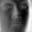
\includegraphics[width=\textwidth]{eigenface2}
            \caption{eigenface 2}
            \label{fig:eigenface2}
        \end{subfigure}
        \caption{Corresponding 3 eigenfaces used for PCA dimensionality reduction.}
        \label{fig:eigenface}
    \end{figure}

    \question PCA plus nearest neighbor classification results

    For classification with PCA, obtain $\mathbf{XV}$, projection of the faces in the test data matrix $\mathbf{X}$ on the
    eigenface space. Each column of $\mathbf{V}$ and therefore each column of $\mathbf{XV}$ corresponds to a principal component.\\
    Again, only calculation for the highest dimension is necessary. The first $k$ projections can be obtained
    with the test data matrix and the first $k$ columns of $\mathbf{V}$.

    It is expected that classfication of selfies is unsuccessful. There are only three selfies in the test
    set and random sampling of 500 images for training included only one selfie which is an outlier in 3D as can be seen from the scatter plots.
    Moreover, my setup and lighting condition differs from those of the images in the PIE data set.

    \begin{center}
        \begin{tabular}{ |c|c|c|c| }
            \hline
            Test Images                & Dimensionality & Accuracy                           \\
            \hline
            \multirow{3}{4em}{CMU PIE} & 40             & \percentage{0.49019607843137253e2} \\
                                       & 80             & \percentage{0.5247058823529411e2}  \\
                                       & 200            & \percentage{0.552156862745098e2}   \\
            \hline
            \multirow{3}{4em}{Selfies} & 40             & \qty{0}{\percent}                  \\
                                       & 80             & \qty{0}{\percent}                  \\
                                       & 200            & \qty{0}{\percent}                  \\
            \hline
        \end{tabular}
    \end{center}

    \question LDA based data distribution visualization
    \question LDA plus nearest neighbor classification results
    \question SVM classification results with different parameter values
    \question CNN classification results with different network architectures

    For CNN, the accuracy ranges from \percentage{0.95e2}to \percentage{0.97} with shuffling of the order of images.

    Following the updated instructions received via email, my model includes two convolutional layers and two fully connected layers.
    The updated number of nodes is ``20-50-500-26''.
    There is an additional scaling layer at the start to scale the range of each pixel from the range \numrange[range-phrase = --]{0}{255} to \numrange[range-phrase = --]{0}{1}.
    Although often recommended, scaling does not seem to improve the classfication accuracy of this model.

    For previous parts of this assignment, labels were taken directly from the folder names in the provided PIE dataset.
    However, for CNN, one hot encoding is necessary because there is no natural ordinal relationship for the order of PIE subjects.
    For classification of two or more labels using one-hot encoded representation, categorical crossentropy is the option in Keras.
    The final layer uses a softmax function to convert logits to probabilities. Otherwise, ReLU is used to introduce nonlinearity.

    The latest optimizer offered by Keras, the AMSGrad variant of ADAM was used for best performance. 
    As ADAM is an adaptive algorithm, no tuning of the learning rate was necessary or offered any improvement to classfication accuracy.

    \begin{footnotesize}
        \begin{verbatim}
        Model: "sequential"
        _________________________________________________________________
         Layer (type)                Output Shape              Param #   
        =================================================================
         rescaling (Rescaling)       (None, 32, 32, 1)         0         
                                                                         
         conv2d (Conv2D)             (None, 28, 28, 20)        520       
                                                                         
         max_pooling2d (MaxPooling2D  (None, 14, 14, 20)       0         
         )                                                               
                                                                         
         conv2d_1 (Conv2D)           (None, 10, 10, 50)        25050     
                                                                         
         max_pooling2d_1 (MaxPooling  (None, 5, 5, 50)         0         
         2D)                                                             
                                                                         
         flatten (Flatten)           (None, 1250)              0         
                                                                         
         dense (Dense)               (None, 500)               625500    
                                                                         
         dense_1 (Dense)             (None, 26)                13026     
                                                                         
        =================================================================
        Total params: 664,096
        Trainable params: 664,096
        Non-trainable params: 0
        _________________________________________________________________
    \end{verbatim}
    \end{footnotesize}


    For simplicity, I arbitrarily set the number epochs to $100$ with batch size of $128$.

    It takes about $55$ epochs to reach \qty{100}{\percent} accuracy on the training set and for the training loss to fall from an initial value of about $3.25$ to $0$.

    \begin{figure}[hb]
        \centering
        \includesvg[width=0.75\textwidth]{epoch_accuracy}
        \caption{Epoch accuracy.}
        \label{fig:epoch_accuracy}
    \end{figure}

    \begin{figure}[htb]
        \centering
        \includesvg[width=0.75\textwidth]{epoch_loss}
        \caption{Epoch loss.}
        \label{fig:epoch_loss}
    \end{figure}
\end{questions}

\end{document}
